\section{Proof of Theorem \ref{thm: main-acm}}\label{sec: proofs}

The goal of this section is to prove Theorem \ref{thm: main-acm} and the subsequent Corollary 
\ref{cor: main-acm-sparse}.
We begin by outlining that the adjusted correlation metric satisfies an approximate triangle inequality in Subsection \ref{sec: tri-ineq}. 
Then in Subsection \ref{sec: lp-norm}, we prove the fractional cost of the adjusted correlation metric in any $\ell_p$-norm objective is an $O(1)$ factor away from the optimal solution's value.
We tie it all together to prove Theorem \ref{thm: main-acm} and Corollary 
\ref{cor: main-acm-sparse} in Subsection \ref{sec: thm1_proof}.

Before all that, we prove a proposition that will be key in several settings. Loosely, it states that if two vertices are close to each other according to $d$, then they have a large shared positive neighborhood. 
 \begin{proposition} \label{prop: pos_overlap}
     Fix vertices $u,v \in V$ and a clustering $\mathcal{C}$ on $V$ such that $d_{uv} \leq 0.7$ and $|N_u^+ \cap C(u)|\hspace{1mm}/ \hspace{1mm} |N_u^+|\geq 0.85$.
     Then $|N_u^+ \cap N_v^+ \cap C(u)| \geq 0.15 \cdot |N_u^+|$.
 \end{proposition}
\begin{proof}
    Since $d_{uv} \leq 0.7$, 
    $\frac{|N_u^+ \cap N_v^+|}{|N_u^+|} \geq \frac{|N_u^+ \cap N_v^+|}{|N_u^+ \cup N_v^+|} \geq 0.3.$
    Using the assumption on $u$ together with the above inequality implies that $|N_v^+ \cap N_u^+ \cap C(u)|\hspace{1mm}/ \hspace{1mm}|N_u^+| \geq 0.85 + 0.3 - 1 = 0.15.$
\end{proof}


\subsection{Triangle inequality}\label{sec: tri-ineq}
Recall that the correlation metric $d$ satisfies the triangle inequality (see Section 4.2 in \cite{DMN23}). We will show that the adjusted correlation metric $f$ satisfies an approximate triangle inequality, which is sufficient for the KMZ rounding algorithm. 
Formally, we say that a function $g$ is a \emph{$\delta$-semi-metric} on some set $S$ if it is a semi-metric on $S$, except instead of satisfying the triangle inequality, $g$ satisfies 
$g(u,v) \leq \delta \cdot( g(u,w) + g(v,w))$ for all $u,v,w \in S$. 


\begin{lemma}[Triangle Inequality] \label{lem: adjusted_tri_ineq}
    The adjusted correlation metric $f$ is a $\frac{10}{7}$-semi-metric. 
\end{lemma}

The proof of Lemma \ref{lem: adjusted_tri_ineq} is straightforward given that $d$ satisfies the triangle inequality; see Appendix \ref{sec: tri_ineq}. 


Lemma 3 in \cite{DMN23} proves that one can input a semi-metric that satisfies an approximate triangle inequality (instead of the exact triangle inequality) to the KMZ rounding algorithm (with some loss in the approximation factor). We summarize the main take-away below.


\begin{lemma}[\cite{DMN23}]\label{lem: apx-tri}
    If $g$ is a $\delta$-semi-metric on the set $V$, instead of a true  semi-metric (i.e., $1$-semi-metric), then the KMZ algorithm loses a factor of $1+\delta+\delta^2+\delta^3+\delta^4$.\footnote{When $\delta =1$, this factor equals 5, which is the loss in the KMZ algorithm.}
\end{lemma}
Since we show in Lemma \ref{lem: adjusted_tri_ineq} that $f$ is a $\frac{10}{7}$-semi-metric,
we lose a factor of 12 in inputting $f$ to the KMZ algorithm (along with the factor loss from the fractional cost).



\subsection{Bounding the fractional cost of $\ell_p$-norms}\label{sec: lp-norm}
This section bounds the fractional cost of the adjusted correlation metric for the $\ell_p$-norms.  The following lemma considers the case where $p=\infty$.  The general case is handled in the subsequent lemma.

\begin{lemma} \label{lem: infty_proof}
    The fractional cost of the adjusted correlation metric $f$ in the $\ell_{\infty}$-norm objective is at most $56 \cdot \textsf{OPT}$, where $\textsf{OPT}$ is the cost of the optimal integral solution in the $\ell_{\infty}$-norm.
\end{lemma}

The lemma follows from the fact that the fractional cost of the correlation metric $d$ in the $\ell_{\infty}$-norm is known to be bounded by \cite{DMN23}, and that it only decreases when $d$ is replaced by $f$ due to Definition \ref{def: adj_corr_metric}. For completeness, we include a proof in Appendix \ref{sec: infty_norm}. 

For finite $p \in \mathbb{R}_{\geq 1}$, our techniques hold for any $\ell_p$-norm, as we only require the convexity of $x^p$. As far as we know, there has been no study initiated on the problem for $0 \leq p<1$.
We use two primary lemmas---one for the positive edge fractional cost and one for the negative edge fractional cost---to show that the adjusted correlation metric well approximates the optimal for general $\ell_p$-norms.




\begin{lemma}\label{lem:lp-bdd}
    The fractional cost of the adjusted correlation metric $f$ in the $\ell_p$-norm objective is a constant factor (independent of $p$) away from the cost of the optimal integral solution in the $\ell_p$-norm.
\end{lemma}
\begin{proof}
Let $y$ be the disagreement vector for an optimal clustering $\mathcal{C}$ in the $\ell_p$-norm, for any $p \in \mathbb{R}_{\geq 1} \cup \{\infty\}$. 
When $p = \infty$, see Lemma \ref{lem: infty_proof}.
For $p\in \mathbb{R}_{\geq 1}$,
by definition $\textsf{OPT}^p = \sum_{w \in V} (y(w))^p,$
and the $p$th power of the fractional cost of $f$ is given by 
\[cost(f)^p = \sum_{u \in V} \Big[ \sum_{v \in N_u^+} f_{uv} + \sum_{v \in N_u^-} (1-f_{uv})\Big]^p.\]
\[\text{Observe that }\quad cost(f)^p \leq 2^p \underbrace{\sum_{u \in V} \Big(\sum_{v \in N_u^+} f_{uv} \Big)^p}_{(S^+)^p} + 2^p \underbrace{\sum_{u \in V} \Big(\sum_{v \in N_u^-} (1-f_{uv}) \Big)^p}_{(S^-)^p}.\]

We refer to bounding $(S^+)^p$ as bounding the fractional cost of the positive edges, and likewise $(S^-)^p$ for the negative edges. 
The first sum, $(S^+)^p$, is bounded in Lemma \ref{lem: lp_bdd-pos} and the second sum, $(S^-)^p$, is bounded in Lemma \ref{lem: lp_bdd-neg}. Using those two bounds, together we have 
$cost(f) \leq [2^p((S^+)^p + (S^-)^p)]^{1/p} \leq 529,$
for $p \in [1, \infty)$. Specifically, the middle term is maximized at $p=1$, giving the bound of 529, and tends to below 214 as $p \rightarrow \infty$. (A more tailored analysis in Appendix \ref{sec:l1-norm} gives a constant of 74 for $p=1$.)
\end{proof}
We note that, as our main interest is determining whether a simultaneous constant approximation is even possible (and a combinatorial one, at that), we did not pay particular attention to optimizing constants, but suspect these could be greatly reduced.

\subsubsection{Fractional cost of positive edges in $\ell_p$-norms} \label{sec: pos_edges_lp}

Bounding the fractional cost of the positive edges in the $\ell_p$-norm will be similar to in the simpler $\ell_1$-norm (see Appendix \ref{sec:l1-norm}), only there will be an extra step in which we apply Jensen's inequality. 
\begin{lemma} \label{lem: lp_bdd-pos}
    For $p \in \mathbb{R}_{\geq 1}$, the fractional cost of the adjusted correlation metric $f$ in the $\ell_p$-norm objective for the set of positive edges is a constant factor approximation to the optimal, i.e.,
    $$(S^+)^p =  \sum_{u \in V} \Big(\sum_{v \in N_u^+} f_{uv} \Big)^p \leq 
2^p \cdot [(8^p/2 +1)((20/3)^p + 2 + 2 \cdot 4^p) + 8^p +1 ] \cdot \textsf{OPT}^p.
$$
\end{lemma}

One of the challenges in bounding the cost of $f$ is that disagreements in the $\ell_p$-norm objective for $p \neq 1$ are asymmetric, in that a disagreeing edge charges $y(u)$ and $y(v)$ (whereas for $p=1$ we can just sum the number of disagreeing edges). Step 3 rounds up the edges incident to $u$ when the tradeoff is good \textit{from $u$'s perspective}. However, an edge $(u,v)$ may be rounded up to 1 when this tradeoff is good from $v$'s perspective, but not from $u$'s perspective. The high-level idea for why this is fine is that if $u$ and $v$ are close under $d$, their positive neighborhoods overlap significantly and, in some average sense, $u$ can charge to $v$. Proving this requires a double counting argument using a bipartite auxiliary graph. If $u$ and $v$ are far under $d$, on the other hand, we can charge to the cost of the correlation metric, which will be bounded on an appropriate subgraph.

The second challenge is showing that the $\ell_p$-norm of the disagreement vector, restricted to vertices $u$ that are made singletons in Step 3, is bounded. This again requires a double counting argument.

\begin{proof}
Fix an optimal clustering $\mathcal{C}$. 
We partition vertices based on membership in $C(u)$ or $\overline{C(u)}$ (as defined in Subsection \ref{sec: notation}). Let $y$ denote the disagreement vector of $\mathcal{C}$. We have
\begin{align*}
    (S^+)^p &= \sum_{u \in V} \Big( \sum_{v \in N_u^+} f_{uv}\Big)^p 
    \leq 2^p \underbrace{\sum_{u \in V} \Big(\sum_{v \in N_u^+ \cap C(u)} f_{uv}\Big)^p}_{S_1^+} + 2^p \underbrace{\sum_{u \in V} \Big(\sum_{v \in N_u^+ \cap \overline{C(u)}} f_{uv}\Big)^p}_{S_2^+}.
\end{align*}
 It is easy to bound $S_2^+$ by using the trivial upper bound $f_{uv} \leq 1$:
\[\boxed{S_2^+ = \sum_{u \in V} \Big(\sum_{v \in N_u^+ \cap \overline{C(u)}} f_{uv}\Big)^p \leq \sum_{u \in V} \Big(\sum_{v \in N_u^+ \cap \overline{C(u)}} 1 \Big)^p \leq \sum_{u \in V} (y(u))^p = \textsf{OPT}^p,}\]
where we have used that every edge $(u,v) \in E^+$ with $v \not \in C(u)$ is a disagreement incident to $u$.

Next, we bound $S_1^+$. Let $R_1$ be the set of $u$ for which Step 3 of Definition \ref{def: adj_corr_metric} applies. For these $u$, we have $f_{uv} = 1$ for all $v \in V \setminus \{u\}$. Let $R_2 = V \setminus R_1$. For $u \in R_2$ and $v \in N_u^+$, we have that either $v\in R_2$, in which case $f_{uv} = d_{uv}$; or $v \in R_1$, in which case $f_{uv}=1$. (Note that $V$ is the disjoint union of $R_1$ and $R_2$.) So 
\begin{align*}S_1^+ = \underbrace{\sum_{u \in R_1} \Big(\sum_{v \in N_u^+ \cap C(u), v \neq u} 1 \Big)^p}_{S_{11}^+} + \underbrace{\sum_{u \in R_2}\Big(\sum_{v \in N_u^+ \cap C(u)} f_{uv}\Big)^p}_{S_{12}^+}, \end{align*}
and in particular 
\begin{align*}
    S_{12}^+ &= \sum_{u \in R_2}\Big(\sum_{v \in N_u^+ \cap C(u) \cap R_1} 1 + \sum_{v \in N_u^+ \cap C(u) \cap R_2} d_{uv} \Big)^p \\
    &= \sum_{u \in R_2}\Big(\sum_{\substack{v \in N_u^+ \cap C(u) \cap R_1\\ d_{uv} \leq 1/4}} 1 + \sum_{\substack{v \in N_u^+ \cap C(u) \cap R_1\\ d_{uv} \geq 1/4}} 1 + \sum_{v \in N_u^+ \cap C(u) \cap R_2} d_{uv} \Big)^p \\
    &\leq \sum_{u \in R_2}\Big(\sum_{\substack{v \in N_u^+ \cap C(u) \cap R_1\\ d_{uv} \leq 1/4}} 1 + \sum_{\substack{v \in N_u^+ \cap C(u) \cap R_1\\ d_{uv} \geq 1/4}} 4 \cdot d_{uv} + \sum_{v \in N_u^+ \cap C(u) \cap R_2} d_{uv} \Big)^p \\
    &\leq \sum_{u \in R_2}\Big(\sum_{\substack{v \in N_u^+ \cap C(u) \cap R_1\\ d_{uv} \leq 1/4}} 1 +  \sum_{v \in N_u^+ \cap C(u)} 4 \cdot d_{uv} \Big)^p 
    \leq 2^p  \underbrace{\sum_{u \in R_2}\Big(\sum_{\substack{v \in N_u^+ \cap R_1\\ d_{uv} \leq 1/4}} 1 \Big)^p}_{S_{13}^+} + 8^p \cdot \underbrace{\sum_{u \in R_2} \Big(\sum_{v \in N_u^+ \cap C(u)}  d_{uv} \Big)^p}_{S_{14}^+}.
\end{align*}
First we will bound $S_{13}^+$. To do so, we will strongly use that $d_{uv} \leq 1/4$ in the inner sum. In particular, we will make use of the following easy proposition. 
\begin{proposition} \label{prop: similar_nbhds}
Let $d$ be the correlation metric, and suppose $d_{uv} \leq 1/4$. Then $|N_u^+| \leq \frac{7}{3} \cdot |N_v^+|$.
\end{proposition}
\begin{proof}[Proof of Proposition \ref{prop: similar_nbhds}]
    Since $d_{uv} \leq 1/4$ implies $1-d_{uv} \geq 3/4$, we see that
    \[\frac{|N_u^+ \cap N_v^+|}{|N_u^+| + |N_v^+| - |N_u^+ \cap N_v^+|} \geq 3/4,\]
    and we complete the proof since
    $7\cdot|N_v^+| \geq 7\cdot|N_u^+ \cap N_v^+| \geq 3\cdot|N_u^+| + 3\cdot|N_v^+| \geq 3\cdot|N_u^+|.$
\end{proof}
Next, we will need to create a bipartite auxiliary graph $H = (R_2, R_1, F)$ with $R_2$ and $R_1$ being the sides of the partition, and $F$ being the edge set. We will then use a double counting argument. Place an edge between $u \in R_2$ and $v \in R_1$ if $uv \in E^+$ and $d_{uv} \leq 1/4$. Then we have precisely that 
\[S_{13}^+ = \sum_{u \in R_2} \text{deg}_{H}(u)^p.\] 
 We will show that 
\begin{equation} \label{eq: aux_desired_bound}
  \boxed{S_{13}^+ = \sum_{u \in R_2} \text{deg}_H(u)^p \leq  4^{p-1} \cdot \sum_{v \in R_1} |N_v^+|^p \leq 4^{p-1} \cdot \left((20/3)^p + 2 + 2 \cdot 4^p \right) \cdot \textsf{OPT}^p}
\end{equation}
where the last bound  follows from Proposition \ref{prop: R1_bounding}, which we establish separately below. We will bound via double counting the quantity $L$, defined below. Let $N_H(\cdot)$ denote the neighborhoods in $H$ of the vertices. 
\begin{align}
    L &:= \sum_{f=uv \in F} \left(\text{deg}_H(u) + \text{deg}_H(v) \right)^{p-1}  
    \leq \sum_{v \in R_1} \sum_{u \in N_{H}(v)} \left(\text{deg}_H(v) + \text{deg}_H(u) \right)^{p-1} \notag \\
    &\leq \sum_{v \in R_1} \sum_{u \in N_{H}(v)} \left( |N_v^+| + |N_u^+| \right)^{p-1}  
    \leq \sum_{v \in R_1} \sum_{u \in N_{H}(v)} 4^{p-1} \cdot |N_v^+|^{p-1} \label{eq: closeness_prop} \\
    &\leq 4^{p-1} \cdot \sum_{v \in R_1} |N_v^+| \cdot |N_v^+|^{p-1} \notag 
    = 4^{p-1} \cdot \sum_{v \in R_1} |N_v^+|^p \notag
\end{align}
 where in (\ref{eq: closeness_prop}) we've used Proposition \ref{prop: similar_nbhds}. Note that $L$ is upper bounded by the right-hand side in (\ref{eq: aux_desired_bound}). Now it just remains to show that $L$ is lower bounded by the left-hand side in (\ref{eq: aux_desired_bound}).
\begin{align*}
    L &= \sum_{f=uv \in F} \left(\text{deg}_H(u) + \text{deg}_H(v) \right)^{p-1} 
    = \sum_{u \in R_2} \sum_{v \in N_H(u)} \left(\text{deg}_H(u) + \text{deg}_H(v) \right)^{p-1} \\
    &\geq \sum_{u \in R_2} \sum_{v \in N_H(u)} \text{deg}_H(u)^{p-1} 
    = \sum_{u \in R_2} \text{deg}_H(u) \cdot \text{deg}_H(u)^{p-1} 
    = \sum_{u \in R_2} \text{deg}_H(u)^{p},
\end{align*}
 which is what we sought to show.
Now we bound $S_{14}^+$. 
\begin{align*}
    S_{14}^+ &\leq \sum_{u \in V} \Bigg(\sum_{v \in N_u^+ \cap C(u)} \frac{|N_u^+ \cap N_v^-| + |N_u^- \cap N_v^+|}{|N_u^+ \cup N_v^+|} \Bigg)^p \\
    &\leq \sum_{u \in V} \Bigg(\sum_{v \in N_u^+} \frac{y(u) + y(v)}{|N_u^+ \cup N_v^+|} \Bigg)^p 
    \leq \sum_{u \in V} |N_u^+|^{p-1} \sum_{v \in N_u^+} \frac{(y(u) + y(v))^p}{|N_u^+ \cup N_v^+|^p} \\
    &\leq 2^p\sum_{u \in V}\sum_{v \in N_u^+} |N_u^+|^{p-1} \cdot \frac{y(u)^p}{|N_u^+ \cup N_v^+|^p} + 2^p\sum_{u \in V}\sum_{v \in N_u^+} |N_u^+|^{p-1} \cdot \frac{y(v)^p}{|N_u^+ \cup N_v^+|^p}. 
\end{align*}
In the second line, the first inequality uses the fact that for $w \in (N_u^+ \cap N_v^-) \cup (N_u^- \cap N_v^+)$, then at least one of $(u,w), (v,w)$ is a disagreement, since $v \in C(u)$ in the inner summation of the first line. The second inequality in the second line uses Jensen's inequality. 

To bound the first double sum above, we use an averaging argument:
$$\sum_{u \in V}\sum_{v \in N_u^+} |N_u^+|^{p-1} \cdot \frac{y(u)^p}{|N_u^+ \cup N_v^+|^p} \leq \sum_{u \in V} \sum_{v \in N_u^+} \frac{y(u)^p}{|N_u^+|} = \sum_{u \in V} y(u)^p = \textsf{OPT}^p.$$
To bound the second double sum, we first have to flip it:
\begin{align*}
\sum_{u \in V}\sum_{v \in N_u^+} |N_u^+|^{p-1} \cdot \frac{y(v)^p}{|N_u^+ \cup N_v^+|^p} &= \sum_{v \in V} \sum_{u \in N_v^+} |N_u^+|^{p-1} \cdot \frac{y(v)^p}{|N_u^+ \cup N_v^+|^p} \\
&\leq \sum_{v \in V} \sum_{u \in N_v^+} |N_u^+|^{p-1} \frac{y(v)^p}{|N_u^+|^{p-1} \cdot |N_v^+|} 
= \sum_{v \in V} y(v)^p = \textsf{OPT}^p.
\end{align*}
\text{In total, we have }
$$\boxed{S_{14}^+ \leq 2 \cdot 2^p \cdot \textsf{OPT}^p = 2^{p+1} \cdot \textsf{OPT}^p}$$ 

$$\text{and } \quad\boxed{S_{12}^+ \leq 2^p \cdot S_{13}^+ + 8^p \cdot S_{14}^+ \leq 2^p \cdot 4^{p-1} \cdot \left((20/3)^p + 2 + 2 \cdot 4^p \right) \cdot \textsf{OPT}^p + 8^p \cdot \textsf{OPT}^p.}$$




Next we turn to bounding $S_{11}^+$. Recall that $R_1 = \{u : |N_u^- \cap \{v: d_{uv} \leq 0.7\}| \geq \frac{10}{3} \cdot \Delta_u\} $ 
and
\[S_{11}^+ \leq \sum_{u \in R_1} |N_u^+ \cap C(u)|^p \leq \sum_{u \in R_1} |N_u^+|^p.\]

So it suffices to bound the right-hand side, which we do in the following proposition. 
\begin{proposition} \label{prop: R1_bounding} Let $R_1$ be the set of $u$ for which Step 3 of Definition \ref{def: adj_corr_metric} applies. Then 
    $$\sum_{u \in R_1} |N_u^+|^p \leq \left((20/3)^p + 2 + 2 \cdot 4^p \right) \cdot \textsf{OPT}^p.$$
\end{proposition}

\begin{proof}[Proof of Proposition \ref{prop: R1_bounding}]
For $u \in R_1$, define 
$R_1(u) = N_u^- \cap \{v: d_{uv} \leq 0.7\},$
so in particular $|R_1(u)| \geq \frac{10}{3} \cdot \Delta_u$. Fix a vertex $u \in R_1$. We consider a few cases. The crux of the argument is Case 2a(ii). 

\paragraph{Case 1: }\emph{At least a 0.15 fraction of $N_u^+$ is in clusters other than $C(u)$.} \\
Let $ u \in V^{1}$ be the vertices in this case.
This means that $0.15 \cdot |N_u^+| \leq y(u)$, so 
\[\boxed{\sum_{u \in V^1} |N_u^+|^p \leq \sum_{u \in V^1} \frac{1}{0.15^p} y(u)^p \leq (20/3)^p \cdot \textsf{OPT}^p.}\]

\paragraph{Case 2: }\emph{At least a 0.85 fraction of $N_u^+$ is in $C(u)$. }\\
We further partition the cases based on how much $R_1(u)$ intersects $C(u)$.\\

\begin{figure}
    \centering
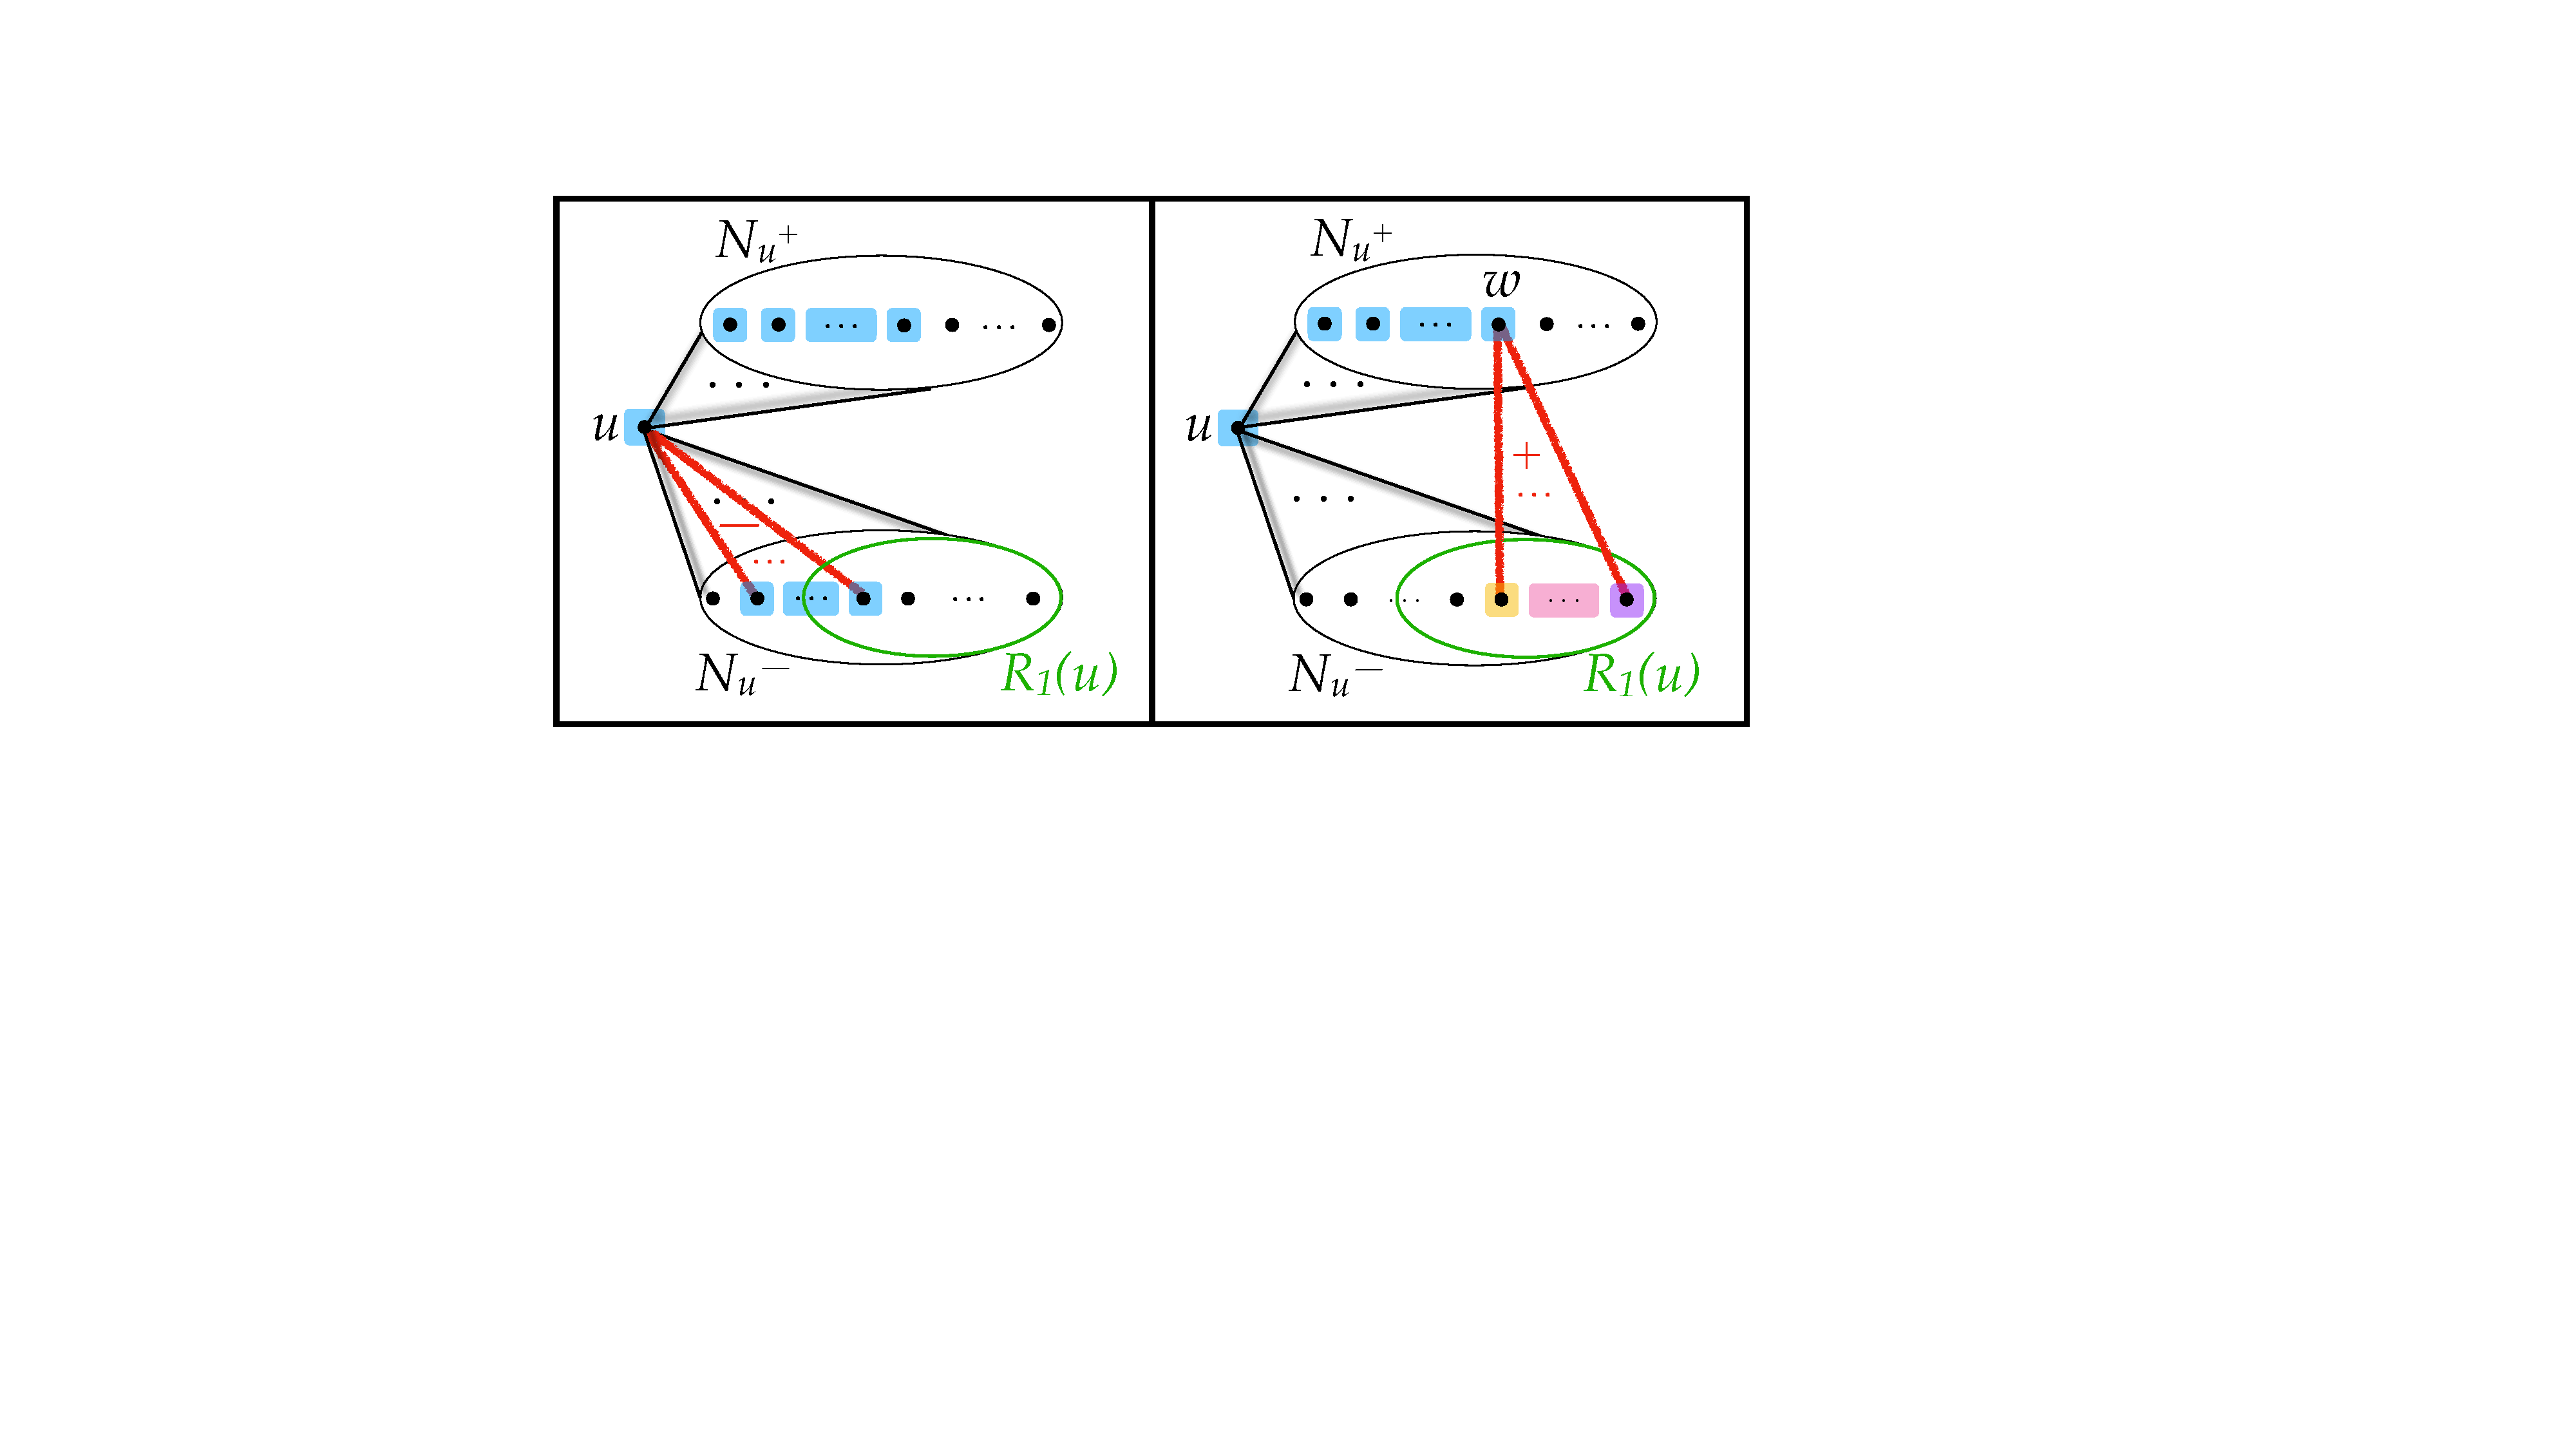
\includegraphics[width = 8cm]{soda-cc-figs-claim2a.pdf}
    \caption{\textbf{Left:} Case 2a(i). For $v \in |N_u^- \cap C(u)|$, $(u,v)$ is a disagreement.
    \textbf{Right:} Case 2a(ii). For $w \in |N_u^+ \cap C(u)|$ and $v \in N_w^+ \cap R_1'(u)$, $(w,v)$ is a disagreement.}
    \label{fig: case2a}
\end{figure}


\noindent\textbf{Case 2a:} \emph{ At least half of $R_1(u)$ is in clusters other than $C(u)$.} \\
We partition into cases (just one more time!) based on the size of $N_u^- \cap C(u)$. See Figure \ref{fig: case2a}.
    \begin{itemize}
        \item \textbf{Case 2a(i):} \emph{At least half of $R_1(u)$ is in clusters other than $C(u)$ and $|N_u^- \cap C(u)| \geq \Delta_u$. }\\
        Let $ u \in  V^{2a(i)}$ be the vertices in this case.
        Note that $y(u) \geq |N_u^- \cap C(u)|$. Then
        \begin{align*}
        \boxed{
        \sum_{ u \in  V^{2ai}} |N_u^+|^p 
        = \sum_{ u \in  V^{2ai}} \Delta_u^p 
        \leq \sum_{ u \in  V^{2ai}} |N_u^- \cap C(u)|^p 
        \leq \sum_{ u \in  V^{2ai}} y(u)^p 
        \leq \textsf{OPT}^p.}
        \end{align*}
        \item \textbf{Case 2a(ii):}\emph{ At least half of $R_1(u)$ is in clusters other than $C(u)$ and $|N_u^- \cap C(u)| \leq \Delta_u$.}\\ 

        Let $ u \in  V^{2a(ii)}$ be the vertices in this case.
    Denote the vertices in $R_1(u)$ that are in clusters other than $C(u)$ by $R_1'(u)$. By definition of Case 2a(ii), $|R_1'(u)| \geq \frac{5}{3} \cdot \Delta_u$. 
        A key fact we will use is that $|C(u)| \leq 2 \cdot \Delta_u$:
        $$|C(u)| = |N_u^- \cap C(u)| + |N_u^+ \cap C(u)| \leq \Delta_u + \Delta_u = 2 \cdot \Delta_u.$$
        For $u \in  V^{2a(ii)}$ and $w \in N_u^+ \cap C(u)$, define 
        $\varphi(u,w) = |R_1'(u) \cap N_w^+|.$


        Each $w \in N_u^+ \cap C(u)$ dispenses 
        $\varphi(u,w)^p/|C(u)|$ charge to $u$. Also, observe that for $v \in R_1'(u)$, we have that $d_{uv} \leq 0.7$, so we know by Proposition \ref{prop: pos_overlap} that $|N_u^+ \cap N_v^+ \cap C(u)| \geq 0.15 \cdot |N_u^+|$. This implies that 
                \begin{align*}\sum_{w \in N_u^+ \cap C(u)} |R_1'(u)  \cap N_w^+|  
                &= \sum_{w \in N_u^+ \cap C(u)} \sum_{v \in R_1'(u)  \cap N_w^+} 1  
                = \sum_{v \in R_1'(u)} \sum_{\underset{ \cap C(u) \cap N_u^+}{w \in  \cap N_v^+}} 1 \\
               & = \sum_{v \in R_1'(u)} | C(u) \cap N_u^+ \cap N_v^+| \geq 
                \sum_{v \in R_1'(u)} 0.15\cdot | N_u^+ | \\
                &= 
                 0.15 \cdot |N_u^+| \cdot |R_1'(u)| \geq 0.15 \cdot \Delta_u \cdot \frac{5}{3}\Delta_u = 0.25 \cdot \Delta_u^2.
                \end{align*}

        First we lower bound the amount of charge each $u$ satisfying Case 2a(ii) receives, which is at least
        \begin{align*}
         \frac{1}{|C(u)|} \sum_{w \in N_u^+ \cap C(u)} \varphi(u,w)^p &\geq \frac{1}{|C(u)|} \cdot \frac{1}{|N_u^+ \cap C(u)|^{p-1}} \cdot \Big(\sum_{w \in N_u^+ \cap C(u)} \varphi(u,w) \Big)^p \\
         &\geq \frac{1}{2\Delta_u} \cdot \frac{1}{\Delta_u^{p-1}} \cdot \Big(0.25\cdot \Delta_u^2 \Big)^p 
         \geq \frac{1}{2} \cdot 0.25^p \cdot |N_u^+|^{p},
         \end{align*}
        where in the first inequality we have applied Jensen's inequality. 
    


    Next we need to upper bound the amount of charge dispensed in total to \textit{all} $u$ satisfying Case 2a(ii). Note by definition that $\varphi(u,w) \leq y(w)$. Each vertex $w \in V$ dispenses at most
    $y(w)^p/|C(u)| = y(w)^p/|C(w)|$
    charge to each $u \in C(w) \cap N_w^+$. So in total each $w$ dispenses at most 
    $|C(w)| \cdot y(w)^p/ |C(w)|  = y(w)^p$
    charge to all $u$ satisfying Case 2a(ii). 

    Now we put together the lower and upper bounds on the total charge dispensed:  
    \begin{align*}
        \sum_{w \in V} y(w)^p &\geq \text{charge dispensed} 
        \geq \sum_{u \in  V^{2a(ii)}} \frac{1}{|C(u)|} \sum_{w \in N_u^+ \cap C(u)} \varphi(u,w)^p 
        \geq \sum_{u \in  V^{2a(ii)}} \frac{1}{2} \cdot 0.25^p \cdot |N_u^+|^p.
    \end{align*}
    \[\text{  In all, } \quad \boxed{\sum_{u \in  V^{2a(ii)}} |N_u^+|^p \leq 2 \cdot 4^p \cdot \sum_{w \in V} y(w)^p \leq 2 \cdot 4^p \cdot \textsf{OPT}^p.}\]

    \end{itemize}

\noindent\textbf{Case 2b: }\emph{At least half of $R_1(u)$ is in $C(u)$.} \\
Let $ u \in  V^{2b}$ be the vertices in this case.
    Denote the vertices in $R_1(u)$ that are in $C(u)$ by $R_1''(u)$. By definition of Case 2b, $|R_1''(u)| \geq \frac{5}{3} \cdot \Delta_u$. Since every vertex in $R''(u)$ is in $N_u^-$, there are at least $|R''(u)|$ disagreements incident to $u$. So
    $y(u) \geq |R''(u)| \geq \frac{5}{3} \cdot \Delta_u,$
     which gives that
    \[ \boxed{\sum_{u \in V^{2b}} |N_u^+|^p = \sum_{u \in V^{2b}} \Delta_u^p \leq \sum_{u \in V^{2b}} y(u)^p \leq \textsf{OPT}^p.}\]
Adding the terms in the boxed expressions across all cases, the proposition follows. 
\end{proof} 
$$
\text{So we have} \quad 
\boxed{S_{11}^+ \leq \sum_{u \in R_1} |N_u^+|^p \leq \left((20/3)^p + 2 + 2 \cdot 4^p \right) \cdot \textsf{OPT}^p.}
$$

Adding together all the cases, we conclude that
$$
    (S^+)^p \leq 2^p \cdot (S_1^+ + S_2^+) 
    \leq 2^p \cdot (S_{11}^+ S_{12^+} + S_2^+) 
    \leq 2^p \cdot [(8^p/2 +1)((20/3)^p + 2 + 2 \cdot 4^p) + 8^p +1 ] \cdot \textsf{OPT}^p.
$$
\end{proof}
\subsubsection{Fractional cost of negative edges in $\ell_p$-norms}
This section bounds the cost of negative edges. The meanings of $\mathcal{C}$, $C(\cdot)$, and $y$ are as in the previous subsection. 
\begin{lemma} \label{lem: lp_bdd-neg}
    For $p \in \mathbb{R}_{\geq 1}$, the fractional cost of the adjusted correlation metric $f$ in the $\ell_p$-norm objective for the set of negative edges is a constant factor approximation to the optimal, i.e.,
   $$(S^-)^p = \sum_{u \in V} \Big(\sum_{v \in N_u^-} (1-f_{uv}) \Big)^p \leq 
2^p ((200/9)^p+1+(10/3)^p+2\cdot (20/3)^p)\cdot \textsf{OPT}^p.
$$
\end{lemma}
\begin{proof}
We have 
\begin{align*}
    (S^-)^p &= \sum_{u \in V} \Big(\sum_{v \in N_u^-} (1-f_{uv}) \Big)^p 
    \leq 2^p \underbrace{\sum_{u \in V} \Big(\sum_{v \in N_u^- \cap C(u)} (1-f_{uv}) \Big)^p}_{S_1^-} + 2^p \underbrace{\sum_{u \in V} \Big(\sum_{v \in N_u^- \cap \overline{C(u)}} (1-f_{uv}) \Big)^p}_{S_2^-}.
\end{align*}

It is easy to bound $S_1^-$ by using the trivial upper bound $1-f_{uv} \leq 1$:

\[\boxed{S_1^- = \sum_{u \in V} \Big(\sum_{v \in N_u^- \cap C(u)} (1-f_{uv}) \Big)^p \leq \sum_{u \in V} \Big(\sum_{v \in N_u^- \cap C(u)} 1 \Big)^p \leq \sum_{u \in V} y(u)^p = \textsf{OPT}^p,}\]
where we have used that every edge $(u,v) \in E^-$ with $v \in C(u)$ is a disagreement incident to $u$. Next, we bound $S_2^-$. Let $R_1$ and $R_2$ be as in the previous subsection: 
$R_1 = \{u : |N_u^- \cap \{v: d_{uv} \leq 0.7\}| \geq \frac{10}{3} \cdot \Delta_u\} $
and $R_2 = V \setminus R_1$. For $u \in R_2$, define 
$$V_u = \{v: v \in N_u^- \cap \overline{C(u)}, d_{uv} \leq 0.7\}.$$
Note that the definition of $V_u$ is the same as $R'_1(u)$ in the previous subsection, 
but here $V_u$ is only defined for $u \in R_2$, while $R'_1(u)$ was defined for $u \in R_1$.
For $u \in R_1$, we have $1-f_{uv} = 0$ for every $v \in V \setminus \{u\}$. So the outer sum in $S_2^-$ only need be taken over $u \in R_2$:
\begin{align*}
    S_2^- &= \sum_{u \in R_2} \Big(\sum_{v \in N_u^- \cap \overline{C(u)}} (1-f_{uv}) \Big)^p 
    \leq \sum_{u \in R_2} \Big(\sum_{\substack{v: v \in N_u^- \cap \overline{C(u)},\\ d_{uv} \leq 0.7} } (1-d_{uv}) \Big)^p 
    \leq \sum_{u \in R_2} |V_u|^p
\end{align*}
In the second equality, we have used that if $u \in R_2$ and $v \in N_u^-$, then $f_{uv} = d_{uv}$, unless $f_{uv}$ was rounded up to 1 in Step 2 of Definition \ref{def: adj_corr_metric} (which happens when $d_{uv} > 0.7$), or $f_{uv}$ was rounded up to 1 in Step 3 (in which case $1-f_{uv} = 0 \leq 1-{d_{uv}}$). 


A key observation is that since $u \in R_2$, it is the case that $|V_u| \leq \frac{10}{3} \cdot \Delta_u$. 

\medskip 

Fix a vertex $u \in R_2$. We consider a few cases. 
\paragraph{Case 1: }\emph{At least a 0.15 fraction of $N_u^+$ is in clusters other than $C(u)$.}\\
Define $V^1$ to be the set of $u \in R_2$ that satisfy Case 1. Then for $u \in V^1$,  $0.15 \cdot |N_u^+| \leq y(u)$, and further
$$|V_u| \leq \frac{10}{3}\Delta_u \leq \frac{1}{0.15}\cdot \frac{10}{3} y(u) = \frac{200}{9}y(u).$$
\text{It follows that } 
$$ \boxed{\sum_{u \in V^1} |V_u|^p \leq (200/9)^p \cdot \sum_{u \in V^1} y(u)^p \leq (200/9)^p \cdot \textsf{OPT}^p.}$$

\paragraph{Case 2: }\emph{At least a 0.85 fraction of $N_u^+$ is in $C(u)$. }\\ 
Define $V^2$ to be the set of $u \in R_2$ that satisfy Case 2. 
Fix $u \in V^2$ and $v \in V_u$. Define $N_{u,v} = N_u^+ \cap N_v^+ \cap C(u)$. Since $d_{uv} \leq 0.7$ and by the assumption of this case, using Proposition \ref{prop: pos_overlap} we have  
$$|N_{u,v}| = |N_u^+ \cap N_v^+ \cap C(u)| \geq 0.15 \cdot \Delta_u.$$
Observe that since $v \not 
\in C(u)$ for $v \in V_u$, $(v,w)$ is a (positive) disagreement for all $w \in N_{u,v}$. 

\noindent  \textbf{Case 2a: }\emph{$|N_u^- \cap C(u)| \geq \Delta_u$.} 

    Define $V^{2a}$ to be the set of $u \in V^2$ that satisfy Case 2a. Since all edges $(u,v)$ with $v \in N_u^- \cap C(u)$ are disagreements, we have $y(u) \geq \Delta_u$. Recalling that $|V_u| \leq \frac{10}{3} \cdot \Delta_u$ for $u \in R_2$, we have
    \[\boxed{\sum_{u \in V^{2a}} |V_u|^p \leq \sum_{u \in V^{2a}} (10/3\cdot\Delta_u)^p \leq (10/3)^p \cdot \sum_{u \in V^{2a}} y(u)^p \leq (10/3)^p \cdot \textsf{OPT}^p.}\]

\noindent \textbf{Case 2b: }\emph{$|C(u)| \leq 2\Delta_u$.} 

    Define $V^{2b}$ to be the $u \in V^2$ satisfying Case 2b. 
    Fix $w \in N_u^+ \cap C(u)$ and $u \in V^{2b}$. Define 
    $$\varphi(u,w) = |V_u \cap N_w^+|,$$
    i.e. $\varphi(u,w)$ is the number of $v \in V_u$ with $w \in N_{u,v}$. 
    Each $w \in N_u^+ \cap C(u)$ dispenses 
    $\frac{\varphi(u,w)^p}{|C(u)|}$
    charge to $u$. Also, 
    \begin{align*}\sum_{w \in N_u^+ \cap C(u)} \varphi(u,w) &= 
    \sum_{w \in N_u^+ \cap C(u)} |V_u \cap N_w^+|
    = \sum_{w \in N_u^+ \cap C(u)} \sum_{v \in V_u\cap N_w^+}1 \\
    &= \sum_{v \in V_u} \sum_{w \in N_{u,v}}1 
    =\sum_{v \in V_u}  |N_{u,v}| \geq |V_u| \cdot 0.15 \cdot \Delta_u.
    \end{align*}
    
    Now we can lower bound the amount of charge each $u$ satisfying Case 2b receives, which is at least
    \begin{align*}
    \frac{1}{|C(u)|} \sum_{w \in N_u^+ \cap C(u)} \varphi(u,w)^p &\geq \frac{1}{|C(u)|} \cdot \frac{1}{|N_u^+ \cap C(u)|^{p-1}} \Big(\sum_{w \in N_u^+ \cap C(u)} \varphi(u,w) \Big)^p \\
    &\geq \frac{1}{2\Delta_u} \cdot \frac{1}{\Delta_u^{p-1}} \left(|V_u| \cdot 0.15\cdot \Delta_u \right)^p 
    = \frac{1}{2} \cdot 0.15^p \cdot |V_u|^p,
    \end{align*}
    where in the first line we used Jensen's inequality. 

    To upper bound the amount of charge dispensed in total to \textit{all} $u$ satisfying Case 2b, first note that $\varphi(u,w) \leq y(w)$. Also, each vertex $w \in V$ only distributes charge to $u \in C(w) \cap N_w^+$, and the amount of charge distributed to each such $u$ is 
    $$\frac{\varphi(u,w)^p}{|C(u)|} = \frac{\varphi(u,w)^p}{|C(w)|} \leq \frac{y(w)^p}{|C(w)|},$$
    so that in total each $w$ dispenses at most 
    $\frac{y(w)^p}{|C(w)|} \cdot |C(w)| \leq y(w)^p$ 
 charge. Putting together the lower and upper bounds on the amount of charge dispensed:
 \begin{align*}
     \sum_{w \in V} y(w)^p &\geq \text{total charge dispensed} 
     \geq \sum_{u \in V^{2b}} \frac{1}{|C(u)|} \sum_{w \in N_u^+ \cap C(u)} \varphi(u,w)^p 
     \geq \sum_{u \in V^{2b}} \frac{1}{2} \cdot 0.15^p \cdot |V_u|^p.
 \end{align*}
 So in all,
 \[\boxed{\sum_{u \in V^{2b}} |V_u|^p \leq 2 \cdot (20/3)^p \cdot \sum_{w \in V} y(w)^p = 2 \cdot (20/3)^p \cdot \textsf{OPT}^p.}\]
Adding together all the cases, we see that
$ (S^-)^p\leq 
2^p ((200/9)^p+1+(10/3)^p+2\cdot (20/3)^p)\cdot \textsf{OPT}^p.
$
 \end{proof}

 \subsection{Proofs of Theorem \ref{thm: main-acm} and Corollary {\ref{cor: main-acm-sparse}}} \label{sec: thm1_proof}

Here we show that Theorem \ref{thm: main-acm} and Corollary \ref{cor: main-acm-sparse} follow directly from the preceding lemmas. 



\begin{proof}[Proof of Theorem \ref{thm: main-acm}]
First we show that Lemma \ref{lem:lp-bdd} implies that the clustering resulting from inputting $f$ into the KMZ rounding algorithm is $O(1)$-approximate in any $\ell_p$-norm. Since the rounding algorithm does not depend on $p$, the clustering will be the same for all $p$. 
Let $\mathcal{C^*}$ be the clustering produced by running the KMZ rounding algorithm with the adjusted correlation metric $f$ as input. Let $\textsf{ALG}(u)$ be the number of edges incident to $u$ that are disagreements with respect to $\mathcal{C}^*$. From \cite{KMZ19} and Lemmas \ref{lem: adjusted_tri_ineq} and \ref{lem: apx-tri}, we have that for every $u \in V$,
$\textsf{ALG}(u) \leq 12 \cdot y_u$
where $y_u$ is as in LP \ref{KMZ_LP} when taking $x=f$. 
So $||y||_p$ is the fractional cost of $f$ in the $\ell_p$-norm. 
In what follows, $||\textsf{ALG}||_p$ is the objective value of $\mathcal{C}^*$ in the $\ell_p$-norm and $\textsf{OPT}(p)$ is the optimal objective value in the $\ell_p$-norm. 
Thus using Lemma \ref{lem:lp-bdd} in the last inequality, we have 
\[||\textsf{ALG}||_p \leq 12 \cdot ||y||_p \leq 12 \cdot 529 \cdot \textsf{OPT}(p) = 6348 \cdot \textsf{OPT}(p).\]


We show the overall run-time is $O(n^\omega)$. Recall from the analysis in \cite{DMN23} that computing the correlation metric takes time $O(n^\omega)$, and the KMZ rounding algorithm takes time $O(n^2)$. We just have to show the post-processing of $d$ in Steps 2 and 3 of Definition \ref{def: adj_corr_metric} that were done in order to obtain the adjusted correlation metric $f$ can be done quickly. Indeed, Step 2 takes $O(n^2)$ time as it simply iterates through the edges. Step 3 also takes $O(n^2)$ time, since it visits each vertex and iterates through the neighbors. Thus, the run-time remains $O(n^\omega)$. 
\end{proof}


\begin{proof}[Proof of Corollary \ref{cor: main-acm-sparse}]
    In \cite{DMN23}, they observe that to reduce the run-time from $O(n^\omega)$ to $O(n\Delta^2 \log n)$ for graphs with maximum positive degree bounded by $\Delta$, one can compute the correlation metric $d$ in $O(n\Delta^2)$ time and then run the KMZ rounding algorithm in $O(n\Delta^2 \log n)$ time (see the proof of Corollary 1.2 in Appendix D of \cite{DMN23}). We need only compute $f_{uv}$ when $f_{uv}<1$. Otherwise, we can handle $f_{uv} = 1$ implicitly. As in \cite{DMN23}, for each $u \in V$, we can maintain a list of  $d_{uv}$ for all $v$ with $d_{uv} < 1$. Computing these lists takes $O(n\Delta^2)$ time in total. (This is because there are at most $\Delta^2$ vertices $v$ that are distance two away from $u$ in the positive subgraph.) Steps 2 and 3 only prune these lists further, since some distances that are below 1 may be raised to 1; importantly, no distance that is already equal to 1 under $d$ will be reduced in Steps 2 and 3. To carry out Step 2, for each vertex $u$ it takes $O(\Delta^2)$ time to iterate through the list for $u$ and raise the appropriate $d_{uv}$ to 1. Similarly, to carry out Step 3, for each vertex $u$ it takes $O(\Delta^2)$ time to determine whether the condition in Step 3 is satisfied; if it is, we just handle the vertex $u$ implicitly, as all distances $f_{uv}$ are set to 1. 

    Since each vertex's list still has size at most $\Delta^2$ after the post-processing in Steps 2 and 3, the KMZ rounding algorithm with $f$ as input takes time $O(n\Delta^2 \log n)$, by the exact same argument as in \cite{DMN23}.  
\end{proof}









